\begin{figure*}[t]
\centering
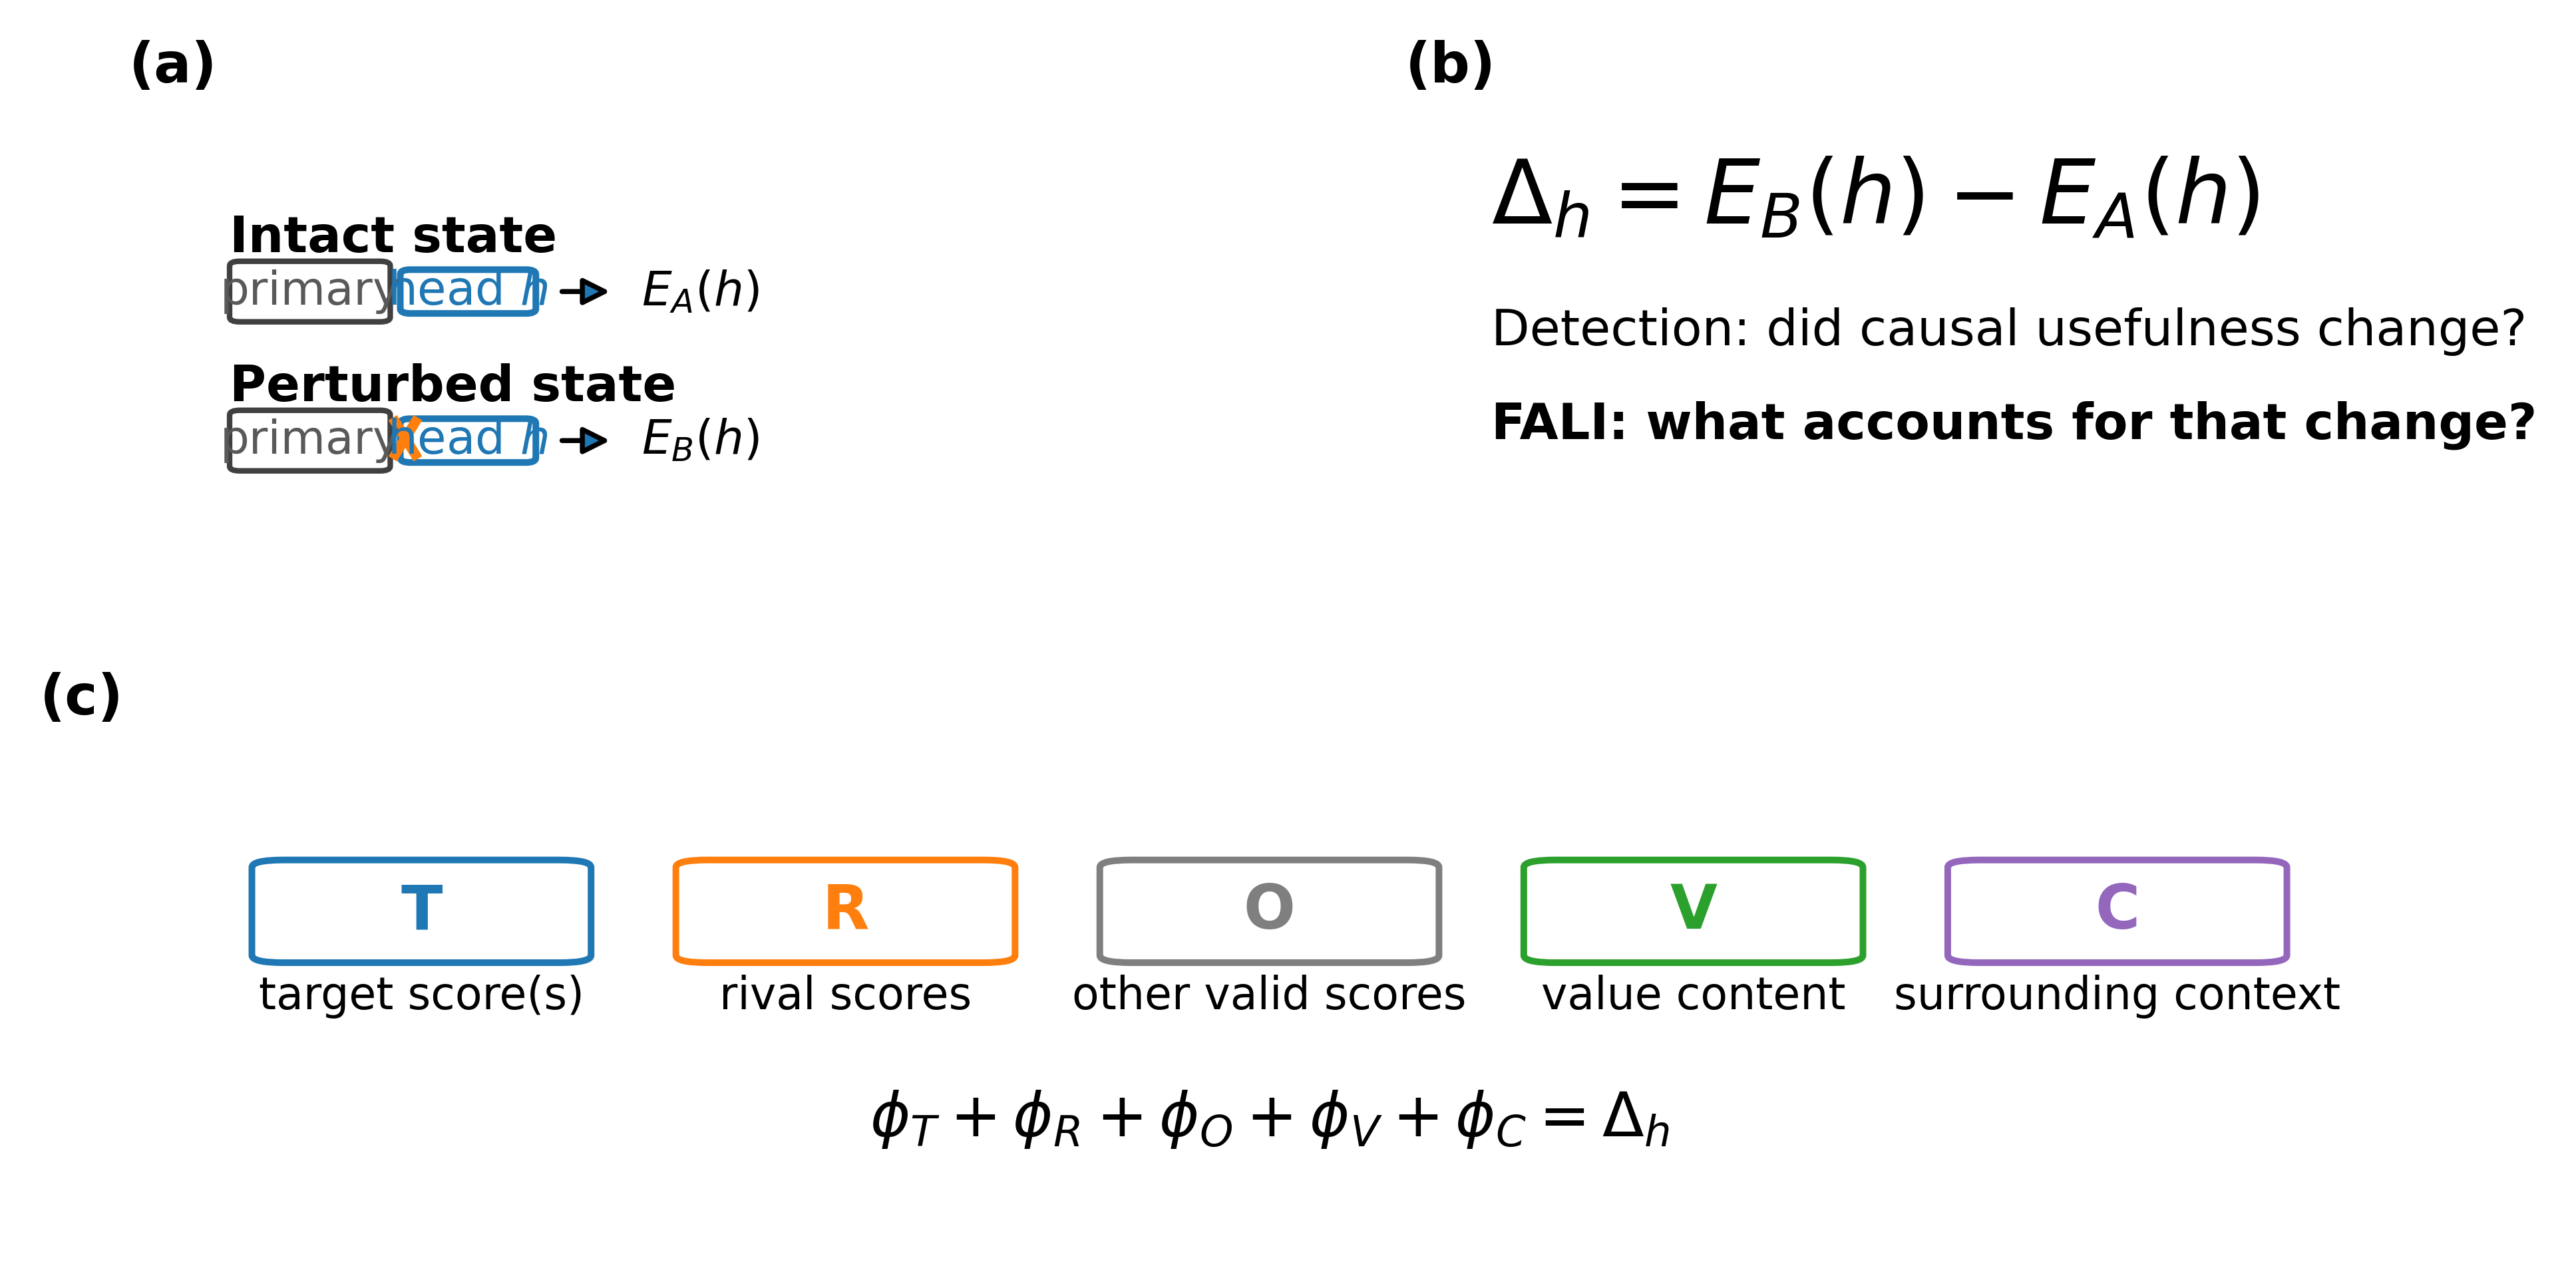
\includegraphics[width=\textwidth]{figures/Fig1.png}
\caption{\textbf{FALI explains a conditional change in candidate-head usefulness.}
The candidate head has output-grounded causal usefulness $E_A(h)$ in the intact context and $E_B(h)$ after the prespecified primary-circuit perturbation, with $\Delta_h=E_B(h)-E_A(h)$ the cross-state change to be explained.
FALI allocates this change among target scores ($T$), rival scores ($R$), other valid scores ($O$), value content ($V$), and surrounding-network context ($C$).
The candidate head and task-relevant target coordinates are specified before FALI analysis; the resulting attributions are defined by the explicit counterfactual intervention game.}
\label{fig:fali-overview}
\end{figure*}
